\Question{Backprop: \emph{Adapted from Fall 2015 Final Exam}}


Suppose we have a neural network that takes in $P = 2000$ input features, has $H = 500$ hidden units, and $N = 4$ outputs.
\begin{figure}[h!]
\begin{center}
  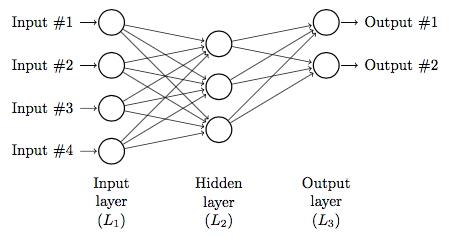
\includegraphics[width=4in]{src/problems/nn/neural_net.png}
  \caption{Network without all input and hidden layer nodes shown}
\end{center}
\end{figure}

$f(x)$ is the activation function in the hidden layer, and $g(x)$ is the activation function in the output layer. You may refer to their respective partial derivatives as $f'(x)$ and $g'(x)$. We will use the mean squared error loss function, which is $L(z) = \frac{1}{2} \| z - y \|^2$ where z is your estimate for label y.\\\\
Let's define some notation! \\
$x\in \mathcal{R}^{P}$ is a feature vector\\
$s^h_j = \sum_{i=1}^{P} V_{i, j}x_i$ are inputs to the hidden layer \\
$h_j = f(s^h_j)$\\
$s^o_k = \sum_{j=1}^{H} W_{j, k}h_j$ are inputs to the output layer\\
$z_k = g(s^o_k)$ \\
$V \in \mathcal{R}^{H\times P}$ are weights between input layer and hidden layer\\
$W \in \mathcal{R}^{N\times H}$ are weights between hidden layer and output layer\\

\begin{Parts}

\Part
Suppose you want to include a bias term in both the input layer and hidden layer, how many weights will be trained? How does this change our weight matrices $V$ and $W$? \\\\
\begin{solution}
$$2001\times 500 + 501\times4 = 1002504$$
Our weight matrices have different dimensions.
$$V \in \mathcal{R}^{H \times (P+1)} \text{ and } W \in \mathcal{R}^{N \times (H+1)}$$
\end{solution}


\Part
Derive the following terms: \\
    \begin{flalign*}
        &\frac{\partial L}{\partial W_{j,k}} = & \\
        &\frac{\partial L}{\partial V_{i,j}} = \\
    \end{flalign*}
\begin{solution}
Back propagation is just a nice term for calculating derivatives using the chain rule. \textbf{The key to using the chain rule in neural networks is to know which variables are related and which variables are independent of each other}. Since $W_{jk}$ is the weight between neuron $h_j$ in the hidden layer and neuron $z_k$ in the output layer, it's important to see $W_{jk}$ and $z_k$ are related while $W_{jk}$ and $z_{k+1}$ are not. By the same reason, 
\begin{align*}
     \frac{\partial L}{\partial W_{j, k}} &= \frac{\partial L}{\partial z_k} \frac{\partial z_k}{\partial s^o_k} \frac{\partial s^o_k}{\partial W_{j, k}} \\
    &= (z_k - y_k) g'(s^o_k) h_j
\end{align*}
In the same way, $V_{ij}$ is the weight between each neuron $x_i$ in the input layer and each neuron $h_j$ in the hidden layer and each $h_j$ affects all the neurons in the output layer. Thus when deriving $\frac{\partial L}{\partial V_{ij}}$, we should apply the chain rule over all output neurons and over only a single neuron $h_j$ in the hidden layer.
\begin{align*}
    \frac{\partial L}{\partial V_{i, j}} &= \sum_{k=1}^N \frac{\partial L}{\partial z_k} \cdot \frac{\partial z_k}{\partial s^o_k} \cdot \frac{\partial s^o_k}{\partial h_j} \cdot \frac{\partial h_j}{\partial s^h_j} \cdot \frac{\partial s^h_j}{\partial V_{i, j}} \\
    &=\sum_{k=1}^N (z_k - y_k) g'(s^o_k) W_{j, k} f'(s^h_j) x_i
\end{align*}
\end{solution}

\Part
As you probably noticed in your homework, vectorizing our backpropagation can speed up computation by taking advantages of matrix operation libraries like numpy. Vectorize the partial derivatives from part (b) and derive the update equation for stochastic gradient descent with learning rate $\eta_1$ and $\eta_2$ for $V$ and $W$. (Use $\otimes$ for elementwise multiplication)

\begin{solution}
Since $\frac{\partial L}{\partial z_k}$ and $\frac{\partial z_k}{\partial s^o_k}$ are associated with subscript $k$, we should apply element wise multiplication between them. Since $\frac{\partial L}{\partial s^o_k}$ and $\frac{\partial s^o_k}{\partial W_{j, k}}$ have different subscript $j$ involved, we should apply matrix multiplication between them.
$$\frac{\partial L}{\partial W} = ((z-y)\otimes g'(S^o))h^\intercal$$

Using similar reason as above, we should apply matrix multiplication between $\frac{\partial L}{\partial s^o_k}$ and $\frac{\partial s^o_k}{\partial h_j}$, element-wise multiplication between $\frac{\partial L}{\partial h_j}$ and $\frac{\partial h_j}{\partial s^h_j}$, matrix multiplication between $\frac{\partial L}{\partial s^h_j}$ and $\frac{\partial s^h_j}{\partial V_{i, j}}$. Note that one should mention $\frac{\partial L}{\partial V} \in \textbf{R}^{500\times 2001}$ in which is all but last row of W in the problem setup since bias term in hidden layer is independent to the values in the input layer.

\begin{align*}
    \\
    \frac{\partial L}{\partial V} &= (W^\intercal ((z-y)\otimes g'(S^o)) \otimes f'(S^h)) x^\intercal
\end{align*}
And the update equations is given by:
\begin{align*}
    V &= V - \eta_1 \frac{\partial L}{\partial V}\\
      &= V - \eta_1 (W^\intercal ((z-y)\otimes g'(S^o)) \otimes f'(S^h)) x^\intercal \\
    W &= W - \eta_2 \frac{\partial L}{\partial W}\\
      &= W - \eta_2 ((z-y)\otimes g'(S^o))h^\intercal\\
\end{align*}
\end{solution}

\Part
The softmax function, or normalized exponential function, is a generalization of the logistic function to handle multiclass classification. The softmax function ``squashes" a N-dimensional vector $s$ of arbitrary real values to a K-dimensional vector $\sigma(s)$ of real values in the range [0, 1] that add up to 1. The $i$-th value corresponds to the probability that the output is class $i$. The function is given by the following:
$$ \sigma(s_j) = \dfrac{e^{s_j}}{\sum_{k=1}^N e^{s_k}} \qquad
\text{ for } j = 1 ... N $$ 

The cross entropy error is commonly paired with softmax activation in the output layer and is defined as:
$$ L(z) = \sum_{k=1}^N y_k \ln (z_k)$$
Now, let $g(x)$ be the softmax function and let our loss function be the cross entropy loss. Calculate the partial derivative of $L$ with respect to $W_{i,j}$.

\begin{solution}
Notice, that our solution from part (b) is no longer accurate because we had assumed $z_k$ did not depend on $W_{i,j}$ if $k \neq j$. However, by the mechanics of the softmax function, that is no longer true, so we have to sum over all $z_k$.
$$ \dfrac{\partial L}{\partial W_{i,j}} = \sum_{k=1}^N \dfrac{\partial L}{\partial z_k} \dfrac{\partial z_k}{\partial s_j} \dfrac{\partial s_j}{\partial W_{i,j}}$$
$$ \dfrac{\partial L}{\partial z_k} = -\dfrac{y_k}{z_k}$$
\[
  \dfrac{\partial z_k}{\partial s_j} =
  \begin{cases}
  z_k(1-z_k)                         & \text{if $i=k$} \\
  -z_i z_k                           & \text{if $i\neq k$}
  \end{cases}
\]
$$ \dfrac{\partial s_j}{\partial W_{i,j}} = h_i $$
\begin{align*}
\dfrac{\partial L}{\partial W_{i,j}} 
&= \sum_{k=1}^N \dfrac{\partial L}{\partial z_k} \dfrac{\partial z_k}{\partial s_j} \dfrac{\partial s_j}{\partial W_{i,j}}\\ 
&= \dfrac{\partial s_j}{\partial W_{i,j}} (\dfrac{\partial L}{\partial z_j} \dfrac{\partial z_j}{\partial s_j} + \sum_{k \neq j}^N \dfrac{\partial L}{\partial z_k} \dfrac{\partial z_k}{\partial s_j})\\
&= \dfrac{\partial s_j}{\partial W_{i,j}} (-\dfrac{y_j}{z_j} z_j(1-z_j) + \sum_{k \neq j}^N -\dfrac{y_k}{z_k} (-z_j z_k))\\
&= \dfrac{\partial s_j}{\partial W_{i,j}} (-y_j (1-z_j) + \sum_{k \neq j}^N  y_k z_j )\\
&= \dfrac{\partial s_j}{\partial W_{i,j}} (-y_j + y_j z_j + \sum_{k \neq j}^N  y_k z_j )\\
&= \dfrac{\partial s_j}{\partial W_{i,j}} (-y_j + \sum_{k = 1}^N  y_k z_j )\\
&= \dfrac{\partial s_j}{\partial W_{i,j}} (-y_j + z_j \sum_{k = 1}^N  y_k  )\\
&= \dfrac{\partial s_j}{\partial W_{i,j}} (-y_j + z_j)\\
&= h_i (-y_j + z_j)\\
\end{align*}

\end{solution}
\end{Parts}

\newpage